\chapter{Preparation}

\section{Segmentation by intensity thresholding}

Before we start the advanced methods of segmentation we will quickly review the simple segmentation strategy of intensity thresholding \cite{bhargavi_survey_2014}.

How does intensity thresholding work? We have an image with a possible range of values between $MIN$ and $MAX$. To apply intensity thresholding we choose in the simplest case one threshold value $t$ with $MIN<=t<=MAX$. All pixels having intensity values $i>=t$ are considered to belong to the foreground, i.e. to the objects of interest, while all pixels with intensity values $i<t$ are considered to be part of the background. This is sufficient when the objects of interest are always higher or lower than the background. But it is not uncommon that the intensities of the objects of interest are in a mid-range of values. In this case we define two threshold values $t_{min}$ and $t_{max}$ and say that all pixels with intensities $i>=t_{min}$ and $i<=t_{max}$ belong to the foreground and all pixels with intensities $i<t_{min}$ or $i>t_{max}$ belong to the background.

All interactive image analysis tools have a tool to set the threshold values. Once the values set, a selection that contains the foreground can easily be created. The foreground can either be selected as one object or each connected part can be selected as a different object. All kinds of features of objects like intensity, area, diameter, perimeter, position and so on can then be measured. If the segmentation needs refinement instead of creating a selection from the threshold values, a binary mask image can be created. Morphological operation like fill holes, dilate, erode, open, close and so on can then be used as post-processing to get a better segmentation. Before doing the segmentation it can be useful to apply filters  to augment the signal/noise ration of the image so that foreground and background can be separated. This comes of course at the cost of smoothing the signal and loosing details of the contour. 

\begin{figure}[h!]
  \centering
\begin{subfigure}[t]{0.3\textwidth}
    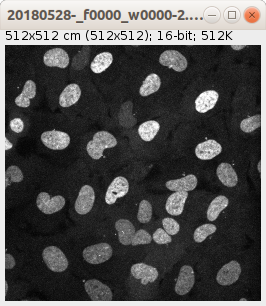
\includegraphics[width=\textwidth]{input-thresholding2}
    \caption[Labeled nuclei]{The input image containing fluorescently labeled nuclei.}
    \label{labeled_nuclei}
\end{subfigure}  
\begin{subfigure}[t]{0.3\textwidth}
    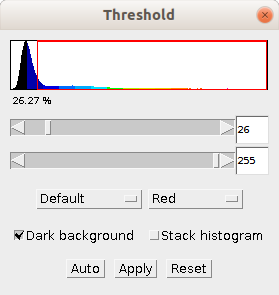
\includegraphics[width=\textwidth]{threshold-adjuster}
    \caption[Threshold Adjuster]{A tool to select the min. and max. threshold values.}
    \label{threshold_adjuster}
\end{subfigure}  
\begin{subfigure}[t]{0.3\textwidth}
    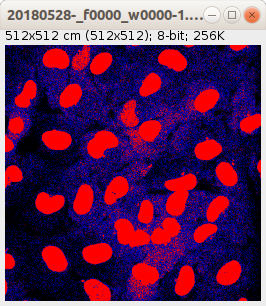
\includegraphics[width=\textwidth]{thresholded02}
    \caption[Segmented image]{Using the threshold values the foreground is displayed in red.}
    \label{segmented_image}
\end{subfigure}  
   \caption{Segmentation by intensity thresholding.}
   \label{segmentation_by_thresholding}
\end{figure}

In Figure \ref{threshold_adjuster} you can see the threshold-adjuster tool from ImageJ \cite{schneider_nih_2012}. On the tool the histogram of the image is displayed. The histogram displays the distribution of the intensity values in the image. On the x-axis are the intensity values eventually divided into a number of intervals (bins) and on the y-axis is the number of times the intensity value (or values in the bin) is present in the image. The histogram can be helpful to find a good threshold value because the foreground and background pixel distribution might be visible in the histogram.

\begin{figure}[h!]
  \centering
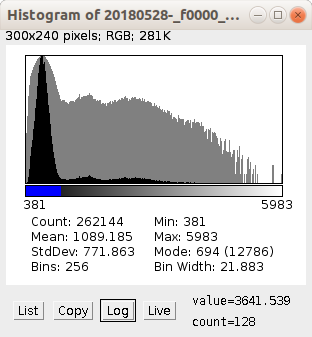
\includegraphics[width=0.4\textwidth]{histogram}
    \caption[histogram]{The histogram after the application of a median filter to the image.}
    \label{histogram}
\end{figure}

In figure \ref{histogram} you can see a peak at the left side that represents the background pixel, while two smaller peaks on the right side are due to the pixels from nuclei. The space between the left peak and the first right peak is due to the out-of-focus nuclei in the image.

\subsection{Global Auto-thresholding}

So far we have chosen the threshold values manually. There are a number of methods to automatically find the threshold values. Most approaches are either based on the histogram of the image or on clustering of intensity values.

\subsubsection{Histogram based methods}

Most histogram based thresholding methods will assume that the distribution of the intensity values has two peaks one representing the background and the other the foreground, i.e. the histogram is bimodal. The threshold should then be in the valley between the two peaks.

As an example we will examine the IsoData algorithm which is also called ''iterative intermeans'' \cite{ridler_picture_1978}. This algorithm repeatedly calculates the average of the means of the values below and above the current threshold estimate until the threshold estimate does not change in the next step:

\begin{enumerate}
\item Select an initial threshold estimate t and set i to 1
\item Let $t_{i}$ be t
\item Calculate the average intensity $L_{i}$ for all intensities below or equal to $t_{i}$
\item Calculate the average intensity $H_{i}$ for all intensities above $t_{i}$
\item Calculate $t_{i+1}$ as the average of $I_{b}$ and $I_{a}$:
\begin{equation}
t_{i+1} = \frac{L_{i} + H_{i}}{2}
\end{equation}
\item If the difference between $t_{i+1}$ and $t_{i}$ is sufficiently small stop and answer $t_{i+1}$, else increment i by one and go to step 3.
\end{enumerate}

\begin{figure}[h!]
  \centering
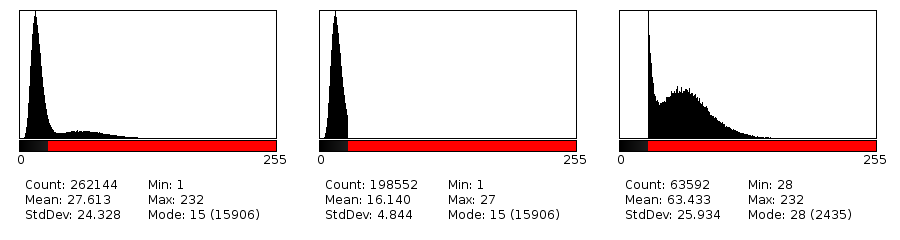
\includegraphics[width=0.95\textwidth]{isoDataHistograms}
    \caption[isoData-histograms]{The initial histogram and the histograms for the parts above and below the initial threshold value. The new threshold value will be $\frac{16+63}{2} = 40$}.
    \label{isoData-histogram}
\end{figure}

\begin{figure}[h!]
  \centering
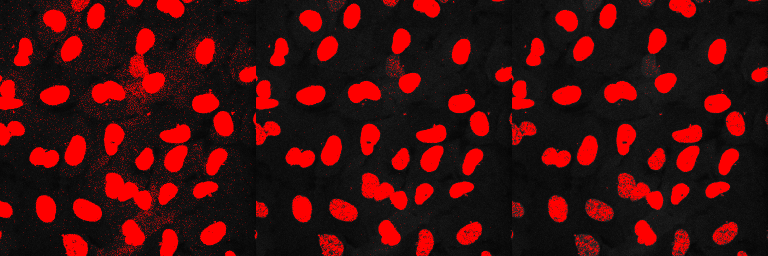
\includegraphics[width=0.95\textwidth]{isoDataThresholds}
    \caption[isoData-segmentation]{Segmentation with the thresholds 28, 40 and 47}.
    \label{isoData-segmentations}
\end{figure}

\subsubsection{Methods based on clustering}

In cluster analysis \cite{tan_introduction_2019}, objects are grouped in a way, that objects which are more similar to one-another fall in the same cluster while objects which are different from each-other belong to different clusters. In our case the objects are intensity values or vectors of intensity values in case of multi-channel images. As a measure of similarity we can for example use the euclidean distance between two intensity values or vectors. 

\paragraph{Otsu Thresholding}

The idea behind Otsu Thresholding \cite{otsu79} is to group objects together in a way that the variance within the groups, the intra-class variance, is minimized. Instead of minimizing the intra-class variance the inter-class variance can be maximized which simplifies the calculation. For an 8-bit image we can easily find the maximum inter-class variation by calculating the inter-class variation for all possible threshold values.

The weighted inter-class variance is given by:

\begin{equation}
	\sigma_{b}^{2}(t) = \omega_{0}(t)\cdot\omega_{1}(t)[\mu_{0}(t) - \mu_{1}(t)]^2
\end{equation}

The weights $\omega_{0}(t)$ and $\omega_{1}(t)$ are the number of intensities below the threshold divided by the total number of intensities and the number of intensities above the threshold divided by the total number of intensities. $\mu_{0}(t)$ and $\mu_{1}(t)$ are the mean-values of the distribution below and above the threshold.

\subsubsection{Adaptive thresholding}

If the illumination of an image is not homogeneous the global threshold will not work satisfactorily. Adaptive thresholding calculates a different threshold for each pixel in the image, depending on the local neighborhood of the pixel. The neighborhood size must be chosen depending on the image, small enough to avoid problems due to inhomogeneous illumination and big enough to contain objects and background.

\section{Separating objects from each other}

In the last chapter we saw how to separate foreground and background of an image by applying a threshold. The result is a binary image that we call a mask. For each pixel it tells us if the pixel belongs to the background or to the foreground. However if we have an image containing multiple cells the binary mask does not tell us to which cell a given pixel belongs. For measuring features of individual objects we need this information. If the objects are separated in the mask the problem is easy to solve:

\begin{enumerate}
\item set the counter to 1
\item for each pixel do
\begin{enumerate}
\item if the pixel belongs to the foreground and has not yet been classified
\begin{enumerate}
\item push the pixel on the stack
\item while the stack is not empty
\begin{enumerate}
\item pop the first pixel p from the stack
\item set the pixel p to counter
\item push all unclassified foreground pixels in the neighborhood of p to the stack
\end{enumerate}
\item increment the counter
\end{enumerate}
\end{enumerate}
\end{enumerate}

For short, this algorithm works in the following way: find a foreground pixel and add all its neighbors and the neighbors of the neighbors and so on to the current class. Then switch to the next class and search for the next yet unclassified foreground pixel.

\begin{figure}[h!]
  \centering
\begin{subfigure}[t]{0.30\textwidth}
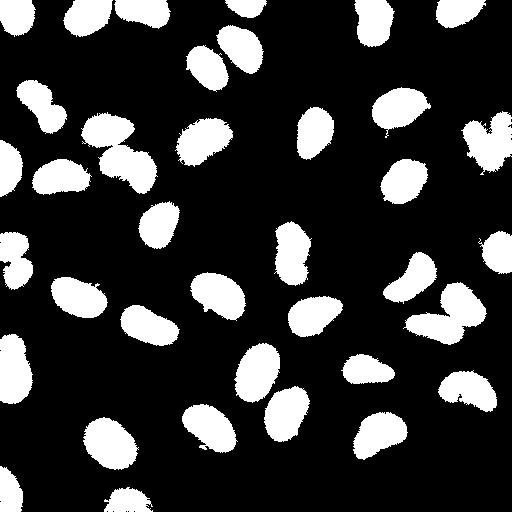
\includegraphics[width=\textwidth]{mask}
    \caption[binary mask]{A binary mask. The image has been divided into foreground and background pixel.}
    \label{binary-mask}
\end{subfigure}  
\begin{subfigure}[t]{0.30\textwidth}

\includegraphics[width=\textwidth]{indexed-mask}
    \caption[indexed mask]{An indexed mask. The background has the value 0 and each pixel has a value that indicates to which object it belongs.}
    \label{indexed-mask}
\end{subfigure}
   \caption{Binary and indexed mask.}
   \label{binary-and-indexed-mask}
\end{figure}

This solves the problem for separated objects. But what if the objects touch each other? 

\subsection{The Watershed Transformation}

To separate objects touching each other the watershed transformation\cite{beucher_morphological_1992} can be used.

To understand the watershed transformation imagine the image as a landscape where regions of high intensity represent mountains and regions of low intensity valleys. Now flip the landscape around so that the mountains become basins and the valleys mountains. Imagine that it is raining on this landscape and that the basins are slowly filling with water. From time to time the waters of to neighboring basins will join as the level of their separation height is reached. Just before this moment we build a dam in the middle between the two basins. These dams are the watershed lines that in the end will partition the whole plane into a number of zones.

The watershed transform can be applied to the greyscale image directly. However without some preprocessing it will usually result in oversegmentation. 

A binary watershed only takes into account the shapes of the objects. In this case the watershed is applied to a distance transform (or distance map) of the binary mask. The distance transform assigns the shortest distance to the border of the object to each pixel within an object and zero to each pixel that does not belong to an object. Different metrics can be used to measure the distance, for example the euclidean metric. In this case we speak of the euclidean distance transform or euclidean distance map.

\begin{figure}[h!]
  \centering
\begin{subfigure}[t]{0.30\textwidth}
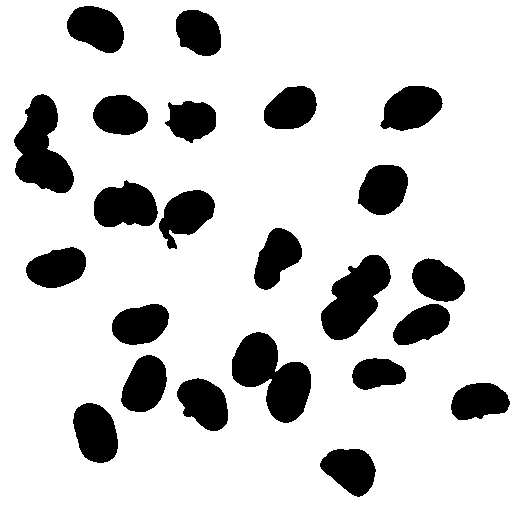
\includegraphics[width=\textwidth]{mask02}
    \caption[A binary mask]{A binary mask of a nuclei image.}
    \label{input-mask}
\end{subfigure}  
\begin{subfigure}[t]{0.30\textwidth}
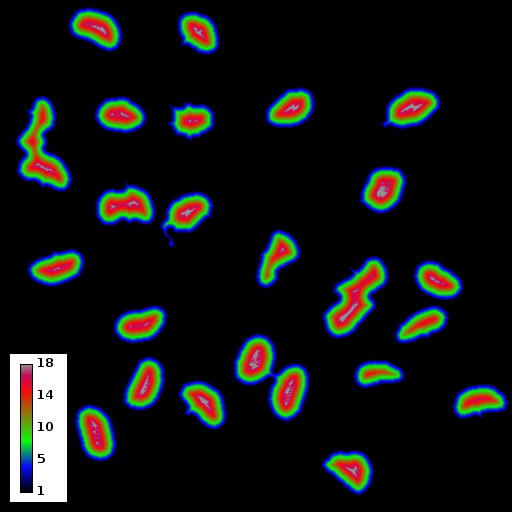
\includegraphics[width=\textwidth]{edm}
    \caption[edm]{The euclidean distance map of the binary mask. The value of each pixel within an object is the shortest distance from the pixel to the border of the object measured with the euclidean distance function.}
    \label{edm}
\end{subfigure}
   \caption{A binary mask and its euclidean distance map.}
   \label{mask-and-edm}
\end{figure}

Figure \ref{basins-and-flooding} shows the euclidean distance map of the input image interpreted as 3D catchment basins. In the flooding process the level of the water raises and just before the water of two basins will mix we draw a dam which defines our watershed line. The dam can be calculated as the voronoi diagram of the two objects. 
 
\begin{figure}[h!]
  \centering
\begin{subfigure}[t]{0.30\textwidth}
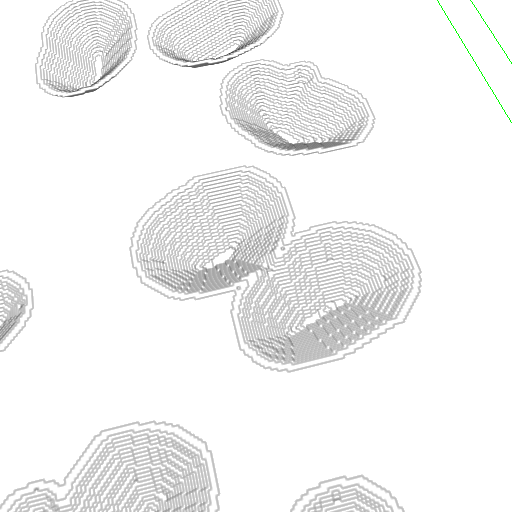
\includegraphics[width=\textwidth]{watershed-basins}
    \caption[Basins]{The distance map interpreted as catchment basins.}
    \label{input-mask}
\end{subfigure}  
\begin{subfigure}[t]{0.30\textwidth}
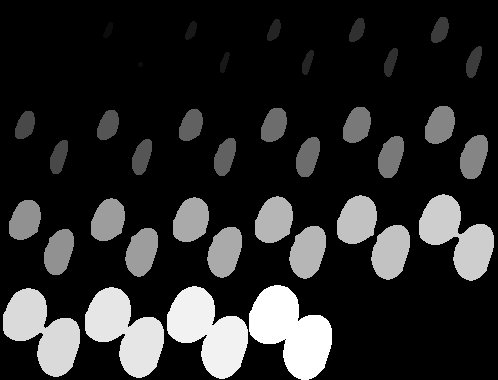
\includegraphics[width=\textwidth]{watershed-montage}
    \caption[Flooding]{Flooding the basins level by level.}
    \label{edm}
\end{subfigure}
   \caption{The catchment basins and the flooding process.}
   \label{basins-and-flooding}
\end{figure}

In a voronoi diagram each pixel is assigned to the closest object. Those pixels that have an equal distance to multiple objects form the dividing lines of the diagram.

\begin{figure}[h!]
  \centering
\begin{subfigure}[t]{0.30\textwidth}
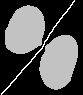
\includegraphics[width=\textwidth]{watershed-before-fusion}
    \caption[Voronoi]{The flooding just before fusion of the basins and the voronoi diagram separating the influence zones.}
    \label{watershed-before-fusion}
\end{subfigure}  
\begin{subfigure}[t]{0.30\textwidth}

\includegraphics[width=\textwidth]{watershed-separation-final}
    \caption[Watershed dam]{The watershed dam, created during the flooding ,separates the touching objects.}
    \label{Watershed dam}
\end{subfigure}
   \caption{The creation of the watershed dam during flooding and separating the touching objects.}
   \label{watershed-dam-final}
\end{figure}

The problem with the watershed transform is that it frequently over-segments the image, i.e. it cuts objects into multiple parts.

\begin{figure}[h!]
  \centering
\begin{subfigure}[t]{0.30\textwidth}
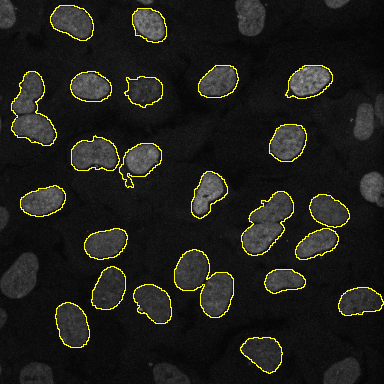
\includegraphics[width=\textwidth]{watershed-nuclei-segmented}
    \caption[Input image for segmentation]{The input image and the objects after thresholding. Some objects are touching each other.}
    \label{watershed-nuclei-segmented}
\end{subfigure}  
\begin{subfigure}[t]{0.30\textwidth}
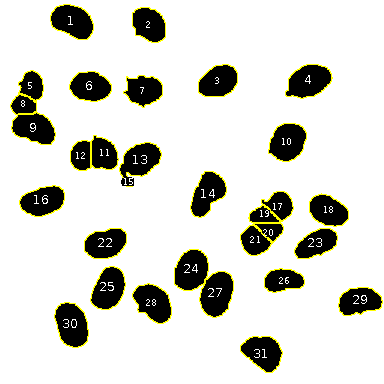
\includegraphics[width=\textwidth]{watershed-result}
    \caption[Watershed result]{Result of the watershed transformation.}
    \label{Watershed result}
\end{subfigure}
   \caption{The watershed has correctly separated the objects 8 and 9, 19 and 20, 24 and 27. But it has also falsely separated 5 and 8, 11 and 12, 20 and 21, 17 and 19.}
   \label{watershed-result-final}
\end{figure}

There are different methods to handle the problem of over-segmentation of the watershed transform. One of them is to use a seeded watershed.